% Notes

% 1 - Find more astro codes that use B-H or FMM


% RESOLVE

% FMM vs tree code terminology
% mention collisional N-body


\documentclass[preprint]{aastex}
\let\captionbox\relax
\usepackage{ulem}
\usepackage{natbib}
\usepackage{morefloats}
\usepackage{amsmath}
\usepackage{graphicx}
\usepackage{verbatim}
\usepackage{color}
\usepackage{ulem}
\usepackage{appendix}
\usepackage{caption}
\usepackage{subcaption}
\usepackage{calc}
\newsavebox\CBox
\newcommand\hcancel[2][0.5pt]{%
  \ifmmode\sbox\CBox{$#2$}\else\sbox\CBox{#2}\fi%
  \makebox[0pt][l]{\usebox\CBox}%  
  \rule[0.5\ht\CBox-#1/2]{\wd\CBox}{#1}}
\bibliographystyle{apj}


\DeclareMathOperator{\arcsinh}{arcsinh}


\begin{document}

\newcommand{\fig}[1]{Figure \ref{#1}}
\newcommand{\eq}[1]{equation (\ref{#1})}
\newcommand{\eqs}[2]{equations (\ref{#1}) - (\ref{#2})}
\newcommand{\Eqs}[2]{Equations (\ref{#1}) - (\ref{#2})}
\newcommand{\vc}[1]{ {\bf{#1}} }
\newcommand{\grad}[1]{ \vc{\nabla } #1 }
\newcommand{\dv}[1]{ \vc{\nabla } \cdot #1 }
\newcommand{\dt}[1]{ \frac{\partial}{\partial t} #1 }
\newcommand{\dx}[2]{ \frac{\partial}{\partial #1} #2 }

\section{Introduction}

\section{Background}
The dynamical stability of the orbits of interacting double white dwarfs (DWDs) depends on the masses of each component white dwarf, whether 
or not the accretion stream directly impacts the surface of the accretor, and the mass loss rate from the system. When mass transfer is unstable,
 the mass transfer rate runs away and the donor is tidally disrupted, resulting in merger. When the mass transfer is stable, long term mass transfer results. 
The latter are thought to form most, if not all, of the population of AM Canum Venaticorum (AM CvN) binaries (cite Kilic et al). \cite{MNS2004} analyze the 
question of stability under the assumption of zero mass loss.

We have used a numerical code to simulate a DWD at the onset of mass transfer. This DWD consists of a 1.0 $M_{\odot}$ CO WD accretor and 0.20 $M_{\odot}$ Roche lobe filling He WD donor with an initial 
separation of $8.85 \times 10^{-2} R_{\odot}$ and an initial orbital period of $242 \mathrm{s}$. 
As can be seen in \fig{mns2004_fig} (Figure 1 from \cite{MNS2004}), this system is just barely in the ``always stable" regime and just barely in the disc accretion regime. 

The orbital angular momentum of two orbiting point masses is given by 
\begin{equation}
\label{jorb}
J_\mathrm{orb} := \sqrt{\frac{G a}{M}} M_1 M_2,
\end{equation}
where $M_1$ and $M_2$ are the masses of each component, $M := M_1 + M_2$, $a$ is the separation, and $J_\mathrm{orb}$ is the orbital angular momentum.
The orbital angular momentum loss rate due to gravitational radiation of two point masses in a circular orbit is given by \cite{P1964},
\begin{equation}
\label{grad}
\dot{J}_\mathrm{orb} = -\frac{32 G^\frac{7}{2} M_1^2 M_2^2 M^\frac{1}{2}}{5 c^5 a^\frac{7}{2} }.
\end{equation}
Using the point mass approximation, we find the logarithmic angular momentum loss rate, $\frac{\dot{J}_\mathrm{orb}}{J_\mathrm{orb}}$, to be $~2 \times 10^{-11} / \mathrm{orbit}$.

Both self-gravitating grid based and and self-gravitating smoothed particle (SPH) based astrophysical codes suffer from violation of angular momentum conservation. Although it is 
possible to preserve angular momentum through the hydrodynamics methods employed by grid based schemes (\cite{BATM2014}, \cite{DL2015}) and by SPH schemes (ADD CITATION), there is no way to 
exactly preserve angular momentum
through the gravitational schemes these methods typically employ. Grid based schemes typically use iterative Poisson solvers and SPH typically uses tree based N-body solvers.
Actual rates of angular momentum violation depend on the particular numerical methods used and what is being modeled.  \cite{MTF2002} found a gain rate of $10^{-4} / \mathrm{orbit}$.
\cite{MT2012} found a loss rate of $10^{-6} / \mathrm{orbit}$ for an interacting binary of mass ratio $0.7$.
\cite{DRGR2011} found a $~10^{-3} / \mathrm{orbit}$ violation rate using SPH to simulate $84$ orbits of an interacting 0.8 $M_{\odot}$ accretor and 0.2 $M_{\odot}$ donor. It is clear that with current
methods it is not possible to reliably simulate a DWD under-going angular momentum driving rates that are anywhere close to the natural angular momentum loss rates due to gravitational radiation.



\section{Numerical Method}



Our numerical code models the self-gravitating three-dimensional inviscid Euler's equations on an AMR mesh. The model equation set is
\begin{equation}
\label{rho_eq}
\dt{\rho_n} + \dv{ \rho_n \vc{v}} = 0,
\end{equation}
\begin{equation} 
\label{mom_eq}
\dt{\vc{s}} + \dv{\vc{v} \vc{s}} + \grad p = \rho \vc{g} +  \vc{\Omega} \times \vc{s},
\end{equation}
\begin{equation} 
\label{lz_eq}
\dt{l_z} + \dv{\vc{v} l_z} + \frac{\partial}{\partial y} x p - \frac{\partial}{\partial x} y p  = x g_y - y g_x,
\end{equation}
\begin{equation} 
\label{etot_eq}
\dt{\left( E + \tfrac{1}{2}\rho\left( \phi -  R^2 \Omega^2 \right) \right) } + \dv{\vc{v} \left( E +  p + \rho \Psi \right)} = \tfrac{1}{2} W_t \left[ \rho, \phi \right] - l_z \dt{\Omega}, 
\end{equation}
\begin{equation}
\label{tau_eq}
\dt{\tau} + \dv{\vc{v} \tau} = 0,
\end{equation}
\begin{equation}
\phi\left[\vc{x}\right] := - \int_V \frac{ G \rho'}{\left| \vc{x} - \vc{x'}\right|} dV',
\end{equation}
\begin{equation}
\dt{\phi}\left[\vc{x}\right] := - \int_V \frac{ G \dt{\rho'}}{\left| \vc{x} - \vc{x'}\right|} dV',
\end{equation}
\begin{equation}
\label{g_eq}
\vc{g} := -\grad{\phi},
\end{equation}
where $\rho_n$ is the mass density of the $n^\mathrm{th}$ species, $\vc{s}$ is the inertial 
frame linear momentum, $l_z$ is the inertial frame $z$-angular momentum, $p$ is the gas pressure,
 $E$ is the rotating frame 
gas energy (including kinetic, internal, and degenerate gas energies), $\vc{R}$ := $x \hat{i} + y \hat{j}$, $\vc{\Omega} := \Omega \hat{k}$ is the angular frequency, $\vc{g}$ is 
the gravitational acceleration, and $\phi$ is the gravitational potential. The Wronskian is defined as 
\begin{equation}
W_t\left[ f_1, f_2 \right] := f_1 \dt{f_2} - f_2 \dt{f_1}.
\end{equation}
The effective potential, $\Psi$, is defined as
\begin{equation}
\Psi := \phi - \tfrac{1}{2} R^2 \Omega^2.
\end{equation} The total density, $\rho$, is the sum of the mass densities of all species,
\begin{equation}
\rho = \Sigma_n \rho_n.
\end{equation} 
For this simulation, we evolve three species, helium, carbon, and oxygen.
The inertial frame
fluid velocity, $\vc{u}$, is defined as 
\begin{equation}
\vc{u} := \frac{\vc{s}}{\rho}.
\end{equation}
It is related to the rotating frame fluid velocity, $\vc{v}$, by the equation
\begin{equation}
\vc{u} := \vc{v} +  \vc{R} \times \vc{\Omega}.
\end{equation}
The pressure, $p$, is determined using the equation of state from \cite{SCM1997}, 
\begin{equation}
p := \left( \gamma - 1\right) \rho \epsilon + p_{\mathrm{deg}}.
\end{equation}
The specific internal gas energy, $\epsilon$, is computed using either the gas energy, $E$, or the ``entropy tracer'', $\tau$, using a variant of the ``dual energy formalism'' (\cite{BNSO1995}). 
First defining a test energy,
\begin{equation}
\epsilon_\mathrm{test} := \frac{1}{\rho}\left( E - \tfrac{1}{2} \rho v^2 - E_\mathrm{deg}  \right), 
\end{equation}
we compute $\epsilon$ using
\begin{equation}
\epsilon :=
\begin{cases}
      \epsilon_\mathrm{test}, & \epsilon_\mathrm{test} > \left ( 1 \times 10^{-3} \right ) \frac{E}{\rho} \\
      \frac{\tau^\gamma}{\rho}, & \text{else}
    \end{cases}.
\end{equation}
The degenerate gas energy and degenerate pressure is computed using the zero temperature equation of state, 
\begin{equation}
E_\mathrm{deg} := A \left \{ 
8 \mathfrak{x}^3 \left ( \sqrt{\mathfrak{x}^2 + 1} - 1 \right )  - P_\mathrm{deg} \right \}
\end{equation}
and
\begin{equation}
P_\mathrm{deg} := A \left \{ 
\mathfrak{x} \left ( 2 \mathfrak{x}^2 - 3 \right ) \sqrt{\mathfrak{x}^2 + 1} + \arcsinh{\mathfrak{x}} \right \}
\end{equation}
respectively, where 
\begin{equation}
\mathfrak{x} := \left( \frac{\rho}{B} \right)^3
\end{equation}
The constants $A$ and $B$ are defined as 
\begin{equation}
A := \frac{\pi m_e^4 c^5}{ 3 h^3 }
\end{equation}
and
\begin{equation}
B := \frac{16 \pi m_p}{ 3 } \left(\frac{m_e c}{ h } \right)^3.
\end{equation}
 

The variables $\rho_n$ and $\tau$ are globally conserved variables, as can be seen by applying Green's theorem to \eq{rho_eq} and \eq{tau_eq}. The conserved energy,  $E_{\mathrm{con}}$, is 
\begin{equation}
E_{\mathrm{con}} := E + \tfrac{1}{2} \rho \left( \phi - R^2 \Omega^2 \right) + l_z \Omega.
\end{equation}
This can be shown by using \eq{lz_eq} to rewrite \eq{etot_eq} as
\begin{equation} 
\label{econ_eq}
\dt{E_{\mathrm{con}} } + \dv{ \left( \vc{v} E_{\mathrm{con}} +  \vc{u} p + \rho \vc{u} \phi \right)} = \tfrac{1}{2} W_t \left[ \rho, \phi \right], 
\end{equation}
Provided $\int_V \vc{s\left({\vc{x}}, t=0\right)} dV = 0$, the second term on the RHS of \eq{mom_eq} globally sums to zero. The gravitational terms on the RHS of \eq{mom_eq} sum to zero when using the
FMM. Using the modification to the FMM described in \S \ref{gsection}, the gravitational term on the RHS \eq{lz_eq} also sums to zero. 
 

\subsection{Initial Conditions}
To generate our initial model, we used a method similar to the self consistent field (SCF) technique described by \cite{ET2009}. The SCF method solves the hydrostatic balance equation in the presence of gravity,
\begin{equation}
h + \Psi = \Psi_0,
\end{equation}
where $\Psi_0$ is a constant unique to each star. The isentropic enthalpy, $h$, is defined as 
\begin{equation}
\label{hbal}
h\left[\rho\right] := \int_0^{P=P\left[\rho\right]} \frac{dP'}{\rho'}.
\end{equation}
For the zero temperature white dwarf equation of state, 
\begin{equation} 
h\left[\rho\right] := \frac{8 A}{B}\sqrt{ \left(\frac{\rho}{B}\right)^\frac{2}{3} + 1} .
\end{equation}

\cite{ET2009} requires the choosing of two boundary points for the donor star, each on the line of centers between the stars and on opposite sides of the donor. For our initial model,
instead of fixing the boundary point closest to the accretor in space, we define it to be the L1 Lagrange point. This sets $\Psi_0$ for the accretor to $\Psi_{L1} + h\left[0\right]$, where $\Psi_{L1}$ is the effective potential at the L1 point. This ensures the donor Roche lobe is filled. The donor white dwarf is taken to be 100 \% hydrogen and the accretor is taken to contain an evenly distributed mixture of 
equal parts of carbon and oxygen.

Because the discretization used for the initial conditions and the discretization that results from writing the time invariant version of the semi-discrete evolution equations are not exactly the same, the initial model is not in exact equilibrium when it begins evolving. As a result, the outer edges of each star diffuse slightly at the very beginning of the simulation. In the case of the donor, this causes Roche lobe overflow, leading to mass transfer.

\subsection {Hydrodyanmics Evolution}
\label{numerical_evolution}

The hydrodynamical variables, $\rho_n$, $\vc{s}$, $\tau$, and $E$, are evolved using the central scheme of \cite{KT2000} (hereafter referred to at ``the KT scheme"). 
In order to conserve $E_{\mathrm{con}}$, we apply the viscosity operator of the KT scheme to the variable $E + \rho \phi - \tfrac{1}{2} \rho R^2 \Omega^2$ (\cite{MT2012}).


As described by \cite{BATM2014}, we evolve $l_z$ on the Cartesian AMR mesh. Along with the modification to the FMM described below in \S \ref{gsection}, this allows for conservation of z-angular momentum
to machine precision (when accounting for flow through the grid boundaries). We evolve $l_z$ in addition to the three components of the momentum vector, $\vc{s}$. At the end of every RK substep, we update
$s_x$ and $s_y$ by first computing the cylindrical radial momentum, 
\begin{equation}
s_R := \frac{x s_x + y s_y}{R},
\end{equation}
and then computing new values for $s_x$ and $s_y$ from $s_R$ and $l_z$, 
\begin{equation}
{s_x}' := \frac{x}{R} s_R - \frac{y}{R^2} l_z,
\end{equation}
\begin{equation}
{s_y}' := \frac{y}{R} s_R + \frac{x}{R^2} l_z.
\end{equation}
This transformation leaves $l_z$ unchanged and results in a $s_R$ that is consistent with the original values for $s_x$ and $s_y$, however, conservation of $s_x$ and $s_y$ are violated. 


The variables on cell faces are obtained by reconstructing the variables are $\rho_n$, $\vc{v}$, $\tau$, $\rho \epsilon$, and $\Phi$ using the piecewise parabolic method (PPM) of \cite{CW1984}. In particular, 
we apply Equation 1.10 of  \cite{CW1984} to all the aforementioned variables, excepting $\Phi$. The gravitational potential, $\Phi$, is presumed smooth and it is reconstructed using Equation 1.9 of \cite{CW1984}.  Prior to the $66^\mathrm{th}$ orbital period, we also apply the PPM reconstruction to $v_\phi := \tfrac{l_z - R \Omega}{\rho R}$. At cell faces the linear momenta, $\vc{s}$, are obtained using reconstructed values for $\vc{v}$, while the inertial frame angular momentum, $l_z$, is obtained using reconstructed values of $v_\phi$. After the $66^\mathrm{th}$ orbital period, the reconstruction of $v_\phi$ is dropped and $l_z$ is computed using $\vc{v}$. 

The set of semi-discrete equations derived from the KT scheme are advanced in time using the third order Runge-Kutta scheme of \cite{SO1988}. 
The quantities $\Phi$, $\dt{\Phi}$, and $\vc{g}$ are computed at each sub-time-step using the method described below in \S \ref{gsection}.

\subsection {Gravity}
\label{gsection}
We depart from typical grid based simulations of astrophysical fluids by using an N-body based solver for the gravitational field. The fast multipole method (FMM), first developed by \cite{GR1997}, is unique among indirect gravity solvers in that it conserves linear momentum to machine precision. Because the long term stability of binary orbits depends on conservation of angular momentum more than linear momentum, we have taken the Cartesian FMM of \cite{D2000} and modified it to conserve z-angular momentum. This modification comes at the expense of violating conservation of x and y linear momentum.


\section{Results}
For purposes of analysis, we separate the computational domain into five distinct regions based on the following criteria:
\begin{equation}
\begin{cases}
      \frac{1}{2} \rho u^2 < \phi 
      \begin{cases}
          x < x_{L1}  
	  \begin{cases}
          	\frac{1}{2} \rho u^2 < 0.1 \phi  \to \mathrm{accretor} \\
          	\frac{1}{2} \rho u^2 \ge 0.1 \phi \to \mathrm{accretor \ disc}
      	  \end{cases}\\
          x \ge x_{L1}  
	  \begin{cases}
          	\frac{1}{2} \rho u^2 < 0.1 \phi  \to \mathrm{donor} \\
          	\frac{1}{2} \rho u^2 \ge 0.1 \phi \to \mathrm{donor \ disc}
      	  \end{cases}\\
      \end{cases}\\
      \frac{1}{2} \rho u^2 < \phi \to \mathrm{unbound}
\end{cases}.
\end{equation}
Here, $x_\mathrm{L2}$ is the $x$ coordinate of the L1 Lagrange point. 

As mentioned in \S \ref{numerical_evolution}, the reconstruction of the inertial angular momentum, $l_z$, is altered in the $66^\mathrm{th}$ orbit. This change results in a small 
shift in the structure of both stars. This effect produces a noticeable artifact in (REFERENCE PLOTS WHERE THIS HAPPENS)

For circular binary orbits, we expect 
\begin{equation}
\label{jdot_eq}
\frac{\dot{J}_{orb}}{J_{orb}} = \frac{\dot{M}_1}{M_1} + \frac{\dot{M}_2}{M_2} + \frac{1}{2} \frac{\dot{a}}{a}
\end{equation}
In \fig{jdot_fig2}, we plot the actual orbit averaged $\frac{\dot{J}_{orb}}{J_{orb}}$ as measured from the simulation output files and  $\frac{\dot{J}_{orb}}{J_{orb}}$ computed using \eq{jdot_eq} and the the
logarithmic time derivatives of $M_1$, $M_2$, and $a$ as determined from the simulation output.

%Assuming synchronous rotation, the spin rotation of the donor may be written as
%\begin{equation}
%J_2 := M_2 i_2 \Omega,
%\end{equation}
%where $i_2$ is the specific moment of inertia for the donor about the z-axis. Because the donor is always filling its Roche lobe, $\frac{\dot{M}_2}{M} >> \frac{\dot{i}_2}{i_2}$, and we may write
%\begin{equation}
%\frac{\dot{J}_2}{J_2} \approx \frac{\dot{M}_2}{M_2} -  \frac{3}{2} \frac{\dot{a}_2}{a_2}.
%\end{equation}

%In \fig{async_fig}, we plot the degree of asynchronous rotation for each star,  ${\Delta \Omega}_1$ and  ${\Delta \Omega}_2$, defined as
%\begin{equation}
%{\Delta \Omega}_{1/2} := \frac{J_{1/2}}{I_{1/2}} - \Omega.
%\end{equation}

\section{Conclusion}


\begin{figure}
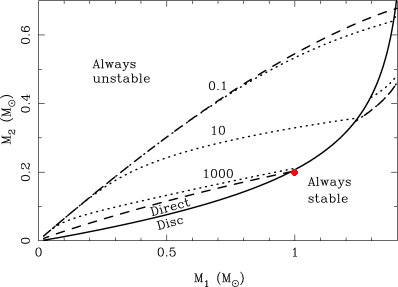
\includegraphics{./images/MNS2004.png}
\caption{This Figure 1 from \cite{MNS2004}, (NOTE: NEED TO ASK PERMISSION), except that we have added a red dot at the location that coincides with our simulated DWD. Systems to the 
left of the left dashed line are always unstable to mass transfer, systems to the right of the right dashed line are always stable, and the stability of systems between the two lines 
depends on the efficiency of the tidal coupling between the two white dwarfs.}
\label{mns2004_fig}
\end{figure}

\begin{figure}
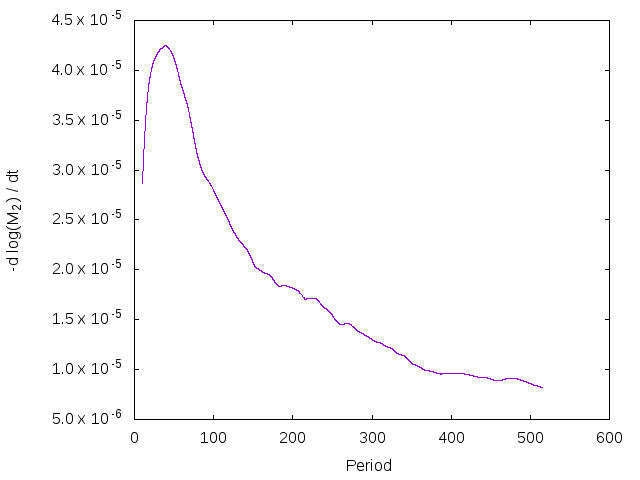
\includegraphics{./images/mdot.png}
\caption{Mass transfer rate}
\label{mdot_fig}
\end{figure}

\begin{figure}
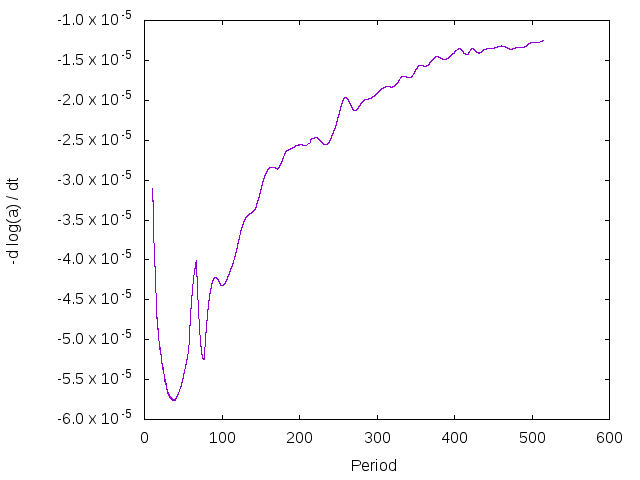
\includegraphics{./images/adot.png}
\caption{Separation change rate}
\label{adot_fig}
\end{figure}

\begin{figure}
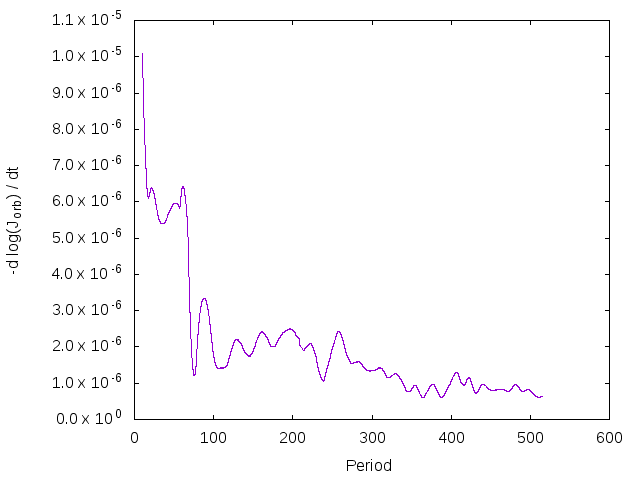
\includegraphics{./images/jdot.png}
\caption{Orbital angular momentum change rate}
\label{jdot_fig}
\end{figure}


\begin{figure}
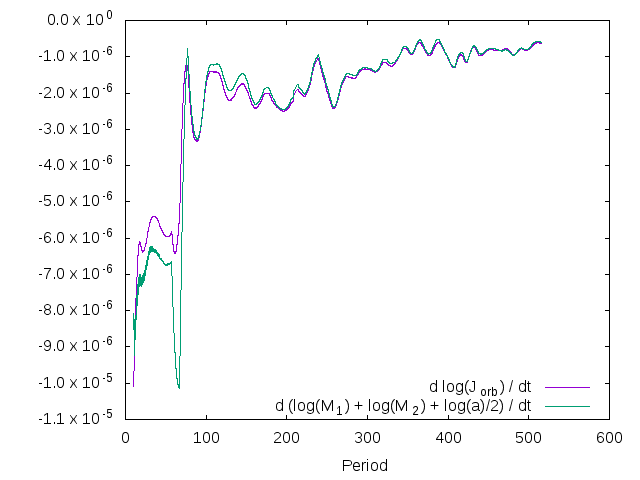
\includegraphics{./images/jorb.png}
\caption{}
\label{jdot_fig2}
\end{figure}

\bibliography{paper}
\end{document}




